%%This is a very basic article template.
%%There is just one section and two subsections.
\documentclass[a4paper]{article}
\usepackage{amssymb}
\usepackage{amsmath}
\usepackage{graphicx}
\usepackage{subfigure}

\begin{document}
	\begin{titlepage}
	
	\centering
	
	{\huge\bfseries Management Dashboard with IBM Cognos\par}
	\vspace{2cm}
	
	
	\begin{figure}
    \subfigure{
\includegraphics[width=0.25\textwidth]{FH}\par\vspace{1cm}}
    \hspace{5cm}
    \subfigure{
\includegraphics[width=0.25\textwidth]{KABEG}\par\vspace{1cm}}
	\end{figure}
	\vspace{1.5cm}
	
	{\Large\itshape Christopher Schmidt and Fabian Matschitsch\par}
	\vfill
	supervised by\par
	Dr.~Florian Hollomey
	ssss
	\vfill
	{\large \today\par}	
	
	\end{titlepage}

	\tableofcontents
	\newpage

	\section{Introduction}
	Hier wird die Einführung stehen.
	\newpage
	
	\section{Hospital Information Communication}
	\subsection{General Communication}
		The general communication for hospital informations is about data of patients,
		medical results, laboratory results, radiographs, financial data, insurance
		data and much more. In the middle of the whole communication will be the
		Hospital Information System (HIS). This system stores the patient information
		and send this data to all other so called Subsystems. A Subsystem will be
		every system which get data from HIS. This systems can also send data back to
		the HIS. For all this communication between the systems there will be a
		standardized protocoll named Health Line 7 (HL7).\\
		The following systems could be subsystems of the Hospital Information System:
		\begin{itemize}
	    	\item Laboratory Information System (LIS)
	    	\item Electronic Medical Record (EMR)
	    	\item Pharmacy Management (PM)
	    	\item Insurance Management (IM)
	    	\item Financial System (FS)
	    	\item Radiology Information System (RIS)
	    	\item Appointment Management (AM)
	    	\item Emergency Management System (EMS)
	    \end{itemize}
	    \begin{figure}[!ht]
		  \centering
		      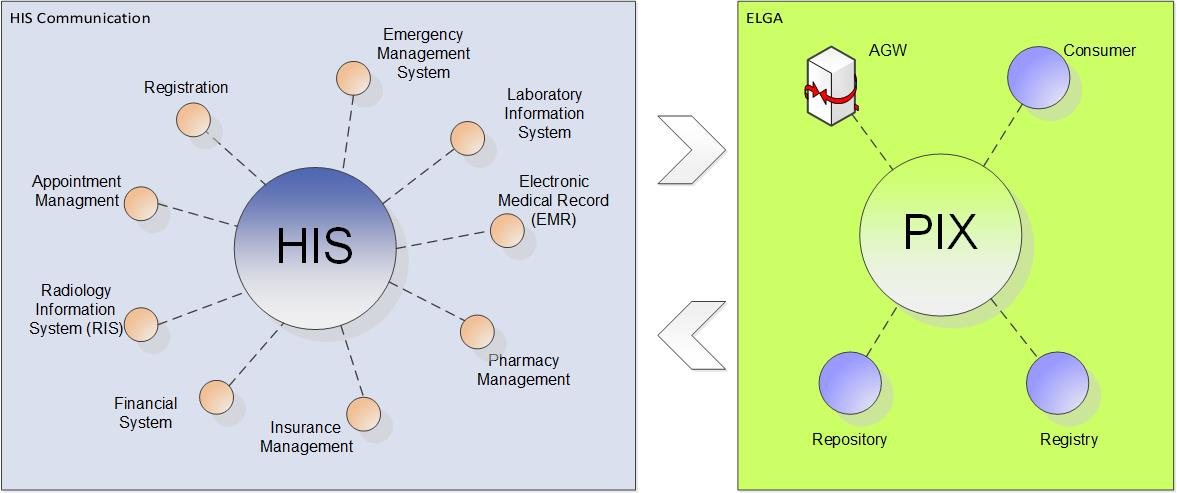
\includegraphics[width=1.0\textwidth]{HIS_Overview}
		  \caption{In the blue box on the left the Hospital Information System
		  Communication is shown. All this system communicate with the ELGA system
		  (on the right) which has an Patient Identifier Cross Referencing (PIX) and
		  an Access Gateway (AGW) for connecting and communicating with external
		  partners.}
		\end{figure}
	    Specially in Austria there will be new kind of system the so called ELGA.
	    This will give the posibility for people in Austria to have a look on their
	    own clinical record in digital way. The ELGA and the system of it will be
	    explained later on in chapter 4.\\
	    To get the systems speaking together a communcation server will be used.
	    This Server connects all the systems together and it is be able to make
	    mappings and database queries to get the right data in the right fields if
	    they are not.
	\subsection{Health Line 7}
		The Health Line 7 (HL7) is a standardized protocol in Version 2.5 and in
		future in Version 3 for the communication in eHealth systems. All systems
		who were communcating in an hospital will be called eHealth systems.\\
		HL7 provides a framework to exchange, integration, sharing and retrieval of
		electronix health information. It defines also the language, structure and the
		data types which are used for the communicatoin between the eHealth systems.\\
		The standard is human-readable and near to all eHealth systems are able to
		read data from HL7 and to export data in HL7.
		
	\newpage
	
	\section{IBM Cognos}
	\subsection{Introduction}
	Introduction to IBM Cognos
	\subsection{Framework Manager}
	Overview to Framework Manager
	\subsection{Report Studio}
	Overview to Report Studio
	\subsection{Data Topology}
	Overview to Data Topology build in Cognos
	
	\newpage
		
	\section{ELGA - Cross Document Sharing}
	\subsection{Weiß nicht genau?}
	\subsection{Next Steps}
	
	\newpage
	
	\section{Hospital Information System - AGFA Orbis}
	The Hospital Information System is the central system in inter-clinical
	communication. In this system all patient data will be stored and every booking
	and terms for the patients will be made.\\
	In the KABEG there are five hospitals and two different Hospital Information
	Systems. In future there should be only one HIS in the KABEG organisation. This
	HIS will be AGFA Orbis.
	\subsection{Orbis in the KABEG}
	At the moment 4 of 5 KABEG hospitals use AGFA Orbis as HIS. The main
	functionality of Orbis is to collect all patient data and sent it to all
	subsystems.
	\subsection{Orbis Database}
	\subsection{Actual Problems}
	\subsection{Reports for Orbis}
	

\end{document}
